\chapter{Sums in Frobenius Algebras} % (fold)
\label{cha:sums_in_frobenius_algebras}
\section{Disjointness in Frobenius Algebras}
\label{sec:disjointness_in_frobenius_algebras}
\begin{definition}\label{def:perp_in_cfrob}
  As shown in ..., $CFrob(\X)$ is a discrete inverse category. For $f,g:A\to B$, define $f\perp g$
  when
\[
\begin{tikzpicture}
\path node at (0,0) [nabla] (n1) {}
node at (0,2.5) (start) {}
node at (-.5,1) [shape=rectangle,draw] (f) {$\scriptstyle f$}
node at (.5,1) [shape=rectangle,draw] (g) {$\scriptstyle g$}
node at (0,2) [delta] (d) {};
\draw [] (d) to (start);
\draw [] (n1) to (0,-0.5);
\draw [] (d) to[out=305,in=90] (g);
\draw [] (d) to[out=235,in=90] (f);
\draw [-] (f) to[out=270,in=125] (n1);
\draw [-] (g) to[out=270,in=65] (n1);
\end{tikzpicture}
\ \raisebox{45pt}{$= 0$}\
\]
\end{definition}

\begin{lemma}\label{lem:cfrobperp_is_a_disjointness_relation}
  The relation $\perp$ of Definition~\ref{def:perp_in_cfrob} is a disjointness relation.
\end{lemma}
\begin{proof}
We need to show the seven axioms of the disjointness relation hold. Note that we will show
\axiom{Dis}{6} early on as its result will be used in some of the other axiom proofs.\\
\axiom{Dis}{1}: For all $f:A\to B,\ f\cdperp 0$.\\
\[
\begin{tikzpicture}
\path node at (0,0) [nabla] (n1) {}
node at (0,2.5) (start) {}
node at (-.5,1) [shape=rectangle,draw] (f) {$\scriptstyle f$}
node at (.5,1) [shape=rectangle,draw] (z) {$\scriptstyle 0$}
node at (0,2) [delta] (d) {};
\draw [] (d) to (start);
\draw [] (n1) to (0,-0.5);
\draw [] (d) to[out=235,in=90] (f);
\draw [] (d) to[out=305,in=90] (z);
\draw [-] (f) to[out=270,in=125] (n1);
\draw [-] (z) to[out=270,in=65] (n1);
\end{tikzpicture}
\ \raisebox{45pt}{$=$}\
\begin{tikzpicture}
\path node at (0,0) [nabla] (n1) {}
node at (0,2.5) (start) {}
node at (-.5,1) [shape=rectangle,draw] (f) {$\scriptstyle f$}
node at (.5,.75) [shape=rectangle,draw] (z) {$\scriptstyle 0$}
node at (.5,1.25) [shape=rectangle,draw] (rz) {$\scriptstyle \rst{0}$}
node at (0,2) [delta] (d) {};
\draw [] (d) to (start);
\draw [] (n1) to (0,-0.5);
\draw [] (d) to[out=235,in=90] (f);
\draw [] (d) to[out=305,in=90] (rz);
\draw [] (rz) to (z);
\draw [-] (f) to[out=270,in=125] (n1);
\draw [-] (z) to[out=270,in=65] (n1);
\end{tikzpicture}
\ \raisebox{45pt}{$=$}\
\begin{tikzpicture}
\path node at (0,0) [nabla] (n1) {}
node at (0,2.75) [shape=rectangle,draw] (tz) {$\scriptstyle 0(=\rst{0})$}
node at (-.5,1) [shape=rectangle,draw] (f) {$\scriptstyle f$}
node at (.5,1) [shape=rectangle,draw] (z) {$\scriptstyle 0$}
node at (0,2) [delta] (d) {};
\draw [] (d) to (tz);
\draw [] (n1) to (0,-0.5);
\draw [] (d) to[out=235,in=90] (f);
\draw [] (d) to[out=305,in=90] (z);
\draw [-] (f) to[out=270,in=125] (n1);
\draw [-] (z) to[out=270,in=65] (n1);
\end{tikzpicture}
\ \raisebox{45pt}{$= 0$}
\]
\axiom{Dis}{6}: $f\cdperp g$ implies $\rst{f} \cdperp \rst{g}$ and $\rg{f}\cdperp\rg{g}$.\\
We will show the details of $\rst{f} \cdperp \rst{g}$, using $\rst{f} = f\inv{f}$ and the definition of
$\inv{f}$ as given in Theorem~\ref{thm:cfrob_is_a_discrete_inverse_category}. The proof of $\inv{f}f
= \rg{f} \perp \rg{g} = \inv{g}g$ is similar.
\[
\begin{tikzpicture}
\path node at (0,0) [nabla] (n1) {}
node at (0,2.5) (start) {}
node at (-.5,1) [shape=rectangle,draw] (f) {$\scriptstyle \rst{f}$}
node at (.5,1) [shape=rectangle,draw] (g) {$\scriptstyle \rst{g}$}
node at (0,2) [delta] (d) {};
\draw [] (d) to (start);
\draw [] (n1) to (0,-0.5);
\draw [] (d) to[out=305,in=90] (g);
\draw [] (d) to[out=235,in=90] (f);
\draw [-] (f) to[out=270,in=125] (n1);
\draw [-] (g) to[out=270,in=65] (n1);
\end{tikzpicture}
\ \raisebox{45pt}{$=$}\
\begin{tikzpicture}
    \path node at (0.5,3.5) [delta] (start) {}
    node at (0,2.5) [eta] (eta1) {}
    node at (0,2) [delta] (d) {}
    node at (-1.2,1.5) [shape=rectangle,draw] (f1) {$\scriptstyle f$}
    node at (-.5,1.5) [shape=rectangle,draw] (f) {$\scriptstyle f$}
    node at (-1,1) [nabla] (n1) {}
    node at (-1,.5) [epsilon] (e1) {}
    node at (2,2.5) [eta] (etag) {}
    node at (2,2) [delta] (dg) {}
    node at (.8,1.5) [shape=rectangle,draw] (g1) {$\scriptstyle g$}
    node at (1.5,1.5) [shape=rectangle,draw] (g) {$\scriptstyle g$}
    node at (1,1) [nabla] (ng) {}
    node at (1,.5) [epsilon] (eg) {}
    node at (1,-.5) [nabla] (end) {};
    \draw [] (start) to[out=235,in=90] (f1);
    \draw [] (start) to[out=305,in=90] (g1);
    \draw [] (f1) to (n1);
    \draw [] (eta1) to (d);
    \draw [] (d) to (end);
    \draw [] (d) to (f);
    \draw [] (f) to (n1);
    \draw [] (n1) to (e1);
    \draw [] (g1) to (ng);
    \draw [] (etag) to (dg);
    \draw [] (dg) to[out=305,in=65] (end);
    \draw [] (dg) to (g);
    \draw [] (g) to (ng);
    \draw [] (ng) to (eg);
\end{tikzpicture}
\ \raisebox{45pt}{$=$}\
\begin{tikzpicture}
    \path node at (0,4) [delta] (start) {}
    node at (-1,3.5) [eta] (eta1) {}
    node at (1,3.5) [eta] (eta2) {}
    node at (-1,3) [delta] (d1) {}
    node at (1,3) [delta] (d2) {}
    node at (-.5,2.5) [nabla] (n1) {}
    node at (.5,2.5) [nabla] (n2) {}
    node at (-.5,2) [shape=rectangle,draw] (f1) {$\scriptstyle f$}
    node at (.5,2) [shape=rectangle,draw] (g2) {$\scriptstyle g$}
    node at (-.5,1.5) [epsilon] (e1) {}
    node at (.5,1.5) [epsilon] (e2) {}
    node at (0,.5) [nabla] (n) {};
    \draw [] (start) to (0,4.5);
    \draw [] (start) to (n1);
    \draw [] (start) to (n2);
    \draw [] (eta1) to (d1);
    \draw [] (eta2) to (d2);
    \draw [] (d1) to[out=235,in=125] (n);
    \draw [] (d1) to (n1);
    \draw [] (d2) to (n2);
    \draw [] (d2) to[out=305,in=65] (n);
    \draw [] (n1) to (f1);
    \draw [] (n2) to (g2);
    \draw [] (f1) to (e1);
    \draw [] (g2) to (e2);
    \draw [] (n)  to (0,0);
\end{tikzpicture}
\ \raisebox{45pt}{$=$}\
\begin{tikzpicture}
    \path node at (0,4) [delta] (start) {}
    node at (-.5,3) [delta] (d1) {}
    node at (.5,3) [delta] (d2) {}
    node at (-.25,2) [shape=rectangle,draw] (f1) {$\scriptstyle f$}
    node at (.25,2) [shape=rectangle,draw] (g2) {$\scriptstyle g$}
    node at (-.25,1.5) [epsilon] (e1) {}
    node at (.25,1.5) [epsilon] (e2) {}
    node at (0,0) [nabla] (n) {};
    \draw [] (start) to (0,4.5);
    \draw [] (start) to (d1);
    \draw [] (start) to (d2);
    \draw [] (d1) to[out=235,in=125] (n);
    \draw [] (d1) to (f1);
    \draw [] (d2) to (g2);
    \draw [] (d2) to[out=305,in=65] (n);
    \draw [] (f1) to (e1);
    \draw [] (g2) to (e2);
    \draw [] (n)  to (0,-.5);
\end{tikzpicture}
\ \raisebox{45pt}{$=$}
\]
\[
\begin{tikzpicture}
    \path node at (0,4) [delta] (start) {}
    node at (.5,3.5) [delta] (d2) {}
    node at (0,2.5) [delta] (d1) {}
    node at (-.25,2) [shape=rectangle,draw] (f1) {$\scriptstyle f$}
    node at (.25,2) [shape=rectangle,draw] (g2) {$\scriptstyle g$}
    node at (0,1.5) [nabla] (n12) {}
    node at (0,1) [epsilon] (e2) {}
    node at (0,0) [nabla] (n) {};
    \draw [] (start) to (0,4.5);
    \draw [] (start) to[out=235,in=125] (n);
    \draw [] (start) to (d2);
    \draw [] (d2) to[out=235,in=90] (d1);
    \draw [] (d1) to (f1);
    \draw [] (d1) to (g2);
    \draw [] (d2) to[out=305,in=65] (n);
    \draw [] (f1) to (n12);
    \draw [] (g2) to (n12);
    \draw [] (n12) to (e2);
    \draw [] (n)  to (0,-.5);
\end{tikzpicture}
\ \raisebox{45pt}{$=$}\
\begin{tikzpicture}
    \path node at (0,3) [delta] (start) {}
    node at (.5,2.5) [delta] (d2) {}
    node at (0,1.75) [shape=rectangle,draw] (z) {$\scriptstyle 0$}
    node at (0,1) [epsilon] (e2) {}
    node at (0,0) [nabla] (n) {};
    \draw [] (start) to (0,3.5);
    \draw [] (start) to[out=235,in=125] (n);
    \draw [] (start) to (d2);
    \draw [] (d2) to[out=235,in=90] (z);
    \draw [] (d2) to[out=270,in=65] (n);
    \draw [] (z) to (e2);
    \draw [] (n)  to (0,-.5);
\end{tikzpicture}
\ \raisebox{45pt}{$=$}\
\begin{tikzpicture}
\path node at (0,0) [nabla] (n1) {}
node at (0,2.5) (start) {}
node at (.5,1) [shape=rectangle,draw] (z) {$\scriptstyle 0$}
node at (0,2) [delta] (d) {};
\draw [] (d) to (start);
\draw [] (n1) to (0,-0.5);
\draw [] (d) to[out=305,in=90] (z);
\draw [] (d) to[out=235,in=125] (n1);
\draw [-] (z) to[out=270,in=65] (n1);
\end{tikzpicture}
\ \raisebox{45pt}{$= 0$}
\]
\axiom{Dis}{2}: $f\cdperp g$ implies $\rst{f} g = 0$.\\
In this proof, we use the result of \axiom{Dis}{6}, i.e., that $\rst{f}\perp\rst{g}$.
\[
\raisebox{25pt}{
\begin{tikzpicture}
  \begin{pgfonlayer}{nodelayer}
    \node [style=map] (0) at (-2, 1) {$\scriptsize \rst{f}$};
    \node [style=map] (1) at (-2, 0) {$\scriptsize g$};
    \end{pgfonlayer}
    \begin{pgfonlayer}{edgelayer}
      \draw (0) to (1);
      \draw (0) to (-2,1.5);
      \draw (1) to (-2, -.5);
      \end{pgfonlayer}
\end{tikzpicture}
}
\ \raisebox{45pt}{$=$}\
\begin{tikzpicture}
  \begin{pgfonlayer}{nodelayer}
    \node [style=map] (0) at (-2, 3) {$\scriptsize \rst{f}$};
    \node [style=map] (1) at (-2, 2.25) {$\scriptsize g$};
    \node [style=delta] (2) at (-1.25, 4) {};
    \node [style=nabla] (3) at (-1.25, 1.25) {};
    \node [style=map] (4) at (-0.5, 3) {$\scriptsize \rst{f}$};
    \node [style=map] (5) at (-0.5, 2.25) {$\scriptsize g$};
    \end{pgfonlayer}
    \begin{pgfonlayer}{edgelayer}
      \draw (0) to (1);
      \draw (1) to[out=270,in=125] (3);
      \draw (5) to[out=270,in=65] (3);
      \draw (4) to (5);
      \draw (2) to[out=305,in=90] (4);
      \draw (2) to[out=235,in=90] (0);
      \draw (2) to (-1.25,4.5);
      \draw (3) to (-1.25,.75);
      \end{pgfonlayer}
\end{tikzpicture}
\ \raisebox{45pt}{$=$}\
\begin{tikzpicture}
  \begin{pgfonlayer}{nodelayer}
    \node [style=map] (0) at (-2, 3) {$\scriptsize \rst{f}$};
    \node [style=map] (1) at (-2, 2.25) {$\scriptsize g$};
    \node [style=delta] (2) at (-1.25, 4) {};
    \node [style=nabla] (3) at (-1.25, 1.25) {};
    \node [style=map] (4) at (-0.5, 2.25) {$\scriptsize g$};
    \end{pgfonlayer}
    \begin{pgfonlayer}{edgelayer}
      \draw (0) to (1);
      \draw (1) to[out=270,in=125] (3);
      \draw (4) to[out=270,in=65] (3);
      \draw (2) to[out=235,in=90] (0);
      \draw (2) to[out=305,in=90] (4);
      \draw (3) to (-1.25,.75);
      \draw (2) to (-1.25,4.5);
      \end{pgfonlayer}
\end{tikzpicture}
\ \raisebox{45pt}{$=$}\
\begin{tikzpicture}
  \begin{pgfonlayer}{nodelayer}
    \node [style=map] (0) at (-2, 2.75) {$\scriptsize \rst{f}$};
    \node [style=map] (1) at (-1.25, 0.75) {$\scriptsize g$};
    \node [style=delta] (2) at (-1.25, 4) {};
    \node [style=nabla] (3) at (-1.25, 1.5) {};
    \node [style=map] (4) at (-0.5, 2.75) {$\scriptsize \rst{g}$};
    \end{pgfonlayer}
    \begin{pgfonlayer}{edgelayer}
      \draw (4) to[out=270,in=65] (3);
      \draw (2) to[out=235,in=90] (0);
      \draw (2) to[out=305,in=90] (4);
      \draw (0) to[out=270,in=125] (3);
      \draw (3) to (1);
      \draw (1) to (-1.25,.25);
      \draw (2) to (-1.25,4.5);
      \end{pgfonlayer}
\end{tikzpicture}
\ \raisebox{45pt}{$=$}\
\raisebox{25pt}{
\begin{tikzpicture}
  \begin{pgfonlayer}{nodelayer}
    \node [style=map] (0) at (-1.25, 1.75) {$\scriptsize 0$};
    \node [style=map] (1) at (-1.25, 0.75) {$\scriptsize g$};
    \end{pgfonlayer}
    \begin{pgfonlayer}{edgelayer}
      \draw (0) to (1);
      \draw (1) to (-1.25,.25);
      \draw (0) to (-1.25,2.25);
      \end{pgfonlayer}
\end{tikzpicture}
}
\ \raisebox{45pt}{$=0$}
\]
\axiom{Dis}{3}: $f\cdperp g,\ f' \le f,\ g' \le g$ implies $f' \cdperp g'$.\\
\[
\begin{tikzpicture}
\path node at (0,0) [nabla] (n1) {}
node at (0,2.5) (start) {}
node at (-.5,1) [shape=rectangle,draw] (f) {$\scriptstyle f'$}
node at (.5,1) [shape=rectangle,draw] (g) {$\scriptstyle g'$}
node at (0,2) [delta] (d) {};
\draw [] (d) to (start);
\draw [] (n1) to (0,-0.5);
\draw [] (d) to[out=305,in=90] (g);
\draw [] (d) to[out=235,in=90] (f);
\draw [-] (f) to[out=270,in=125] (n1);
\draw [-] (g) to[out=270,in=65] (n1);
\end{tikzpicture}
\ \raisebox{45pt}{$=$}\
\begin{tikzpicture}
  \begin{pgfonlayer}{nodelayer}
    \node [style=map] (0) at (-2, 3) {$\scriptsize \rst{f'}$};
    \node [style=map] (1) at (-2, 2.25) {$\scriptsize f$};
    \node [style=delta] (2) at (-1.25, 4) {};
    \node [style=nabla] (3) at (-1.25, 1.25) {};
    \node [style=map] (4) at (-0.5, 3) {$\scriptsize \rst{g'}$};
    \node [style=map] (5) at (-0.5, 2.25) {$\scriptsize g$};
    \end{pgfonlayer}
    \begin{pgfonlayer}{edgelayer}
      \draw (0) to (1);
      \draw (1) to[out=270,in=125] (3);
      \draw (5) to[out=270,in=65] (3);
      \draw (4) to (5);
      \draw (2) to[out=305,in=90] (4);
      \draw (2) to[out=235,in=90] (0);
      \draw (2) to (-1.25,4.5);
      \draw (3) to (-1.25,.75);
      \end{pgfonlayer}
\end{tikzpicture}
\ \raisebox{45pt}{$=$}\
\begin{tikzpicture}
\path
node at (0,3) (start) {}
node at (0,2.5) [shape=rectangle,draw] (fg) {$\scriptstyle \rst{f'}\,\rst{g'}$}
node at (0,2) [delta] (d) {}
node at (-.5,1) [shape=rectangle,draw] (f) {$\scriptstyle f$}
node at (.5,1) [shape=rectangle,draw] (g) {$\scriptstyle g$}
 node at (0,0) [nabla] (n1) {};
\draw [] (d) to (fg);
\draw [] (start) to (fg);
\draw [] (n1) to (0,-0.5);
\draw [] (d) to[out=305,in=90] (g);
\draw [] (d) to[out=235,in=90] (f);
\draw [-] (f) to[out=270,in=125] (n1);
\draw [-] (g) to[out=270,in=65] (n1);
\end{tikzpicture}
\ \raisebox{45pt}{$=$}\
\raisebox{25pt}{
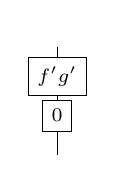
\begin{tikzpicture}
\path
node at (0,1.5) (start) {}
node at (0,1) [shape=rectangle,draw] (fg) {$\scriptstyle \rst{f'}\rst{g'}$}
node at (0,.5) [shape=rectangle,draw] (z) {$\scriptstyle 0$};
\draw [] (z) to (fg);
\draw [] (start) to (fg);
\draw [] (z) to (0,0);
\end{tikzpicture}
}
\ \raisebox{45pt}{$=0$}
\]
\axiom{Dis}{4}: $f\cdperp g$ implies $g \cdperp f$.\\
This follows directly from the co-commutativity of $\Delta$.
\axiom{Dis}{5}: $f\cdperp g$ implies $h f \cdperp h g$.\\
This follows directly from the naturality of $\Delta$.
\axiom{Dis}{7}: $\rst{f}\cdperp \rst{g},\ \rg{h}\cdperp \rg{k}$ implies $f h \cdperp g k$.\\
\[
\begin{tikzpicture}
\path node at (0,0) [nabla] (n1) {}
node at (0,2.5) (start) {}
node at (-.5,1) [shape=rectangle,draw] (fh) {$\scriptstyle f h$}
node at (.5,1) [shape=rectangle,draw] (gk) {$\scriptstyle g k$}
node at (0,2) [delta] (d) {};
\draw [] (d) to (start);
\draw [] (n1) to (0,-0.5);
\draw [] (d) to[out=305,in=90] (gk);
\draw [] (d) to[out=235,in=90] (fh);
\draw [-] (fh) to[out=270,in=125] (n1);
\draw [-] (gk) to[out=270,in=65] (n1);
\end{tikzpicture}
\ \raisebox{45pt}{$=$}\
\begin{tikzpicture}
\path node at (0,0) [nabla] (n1) {}
node at (0,2.5) (start) {}
node at (-.5,1.5) [shape=rectangle,draw] (rf) {$\scriptstyle \rst{f}$}
node at (-.5,1) [shape=rectangle,draw] (fh) {$\scriptstyle f h$}
node at (-.5,.5) [shape=rectangle,draw] (rngh) {$\scriptstyle \rg{h}$}
node at (.5,1.5) [shape=rectangle,draw] (rg) {$\scriptstyle \rst{g}$}
node at (.5,1) [shape=rectangle,draw] (gk) {$\scriptstyle g k$}
node at (.5,.5) [shape=rectangle,draw] (rngk) {$\scriptstyle \rg{k}$}
node at (0,2) [delta] (d) {};
\draw [] (d) to (start);
\draw [] (n1) to (0,-0.5);
\draw [] (d) to[out=305,in=90] (rg);
\draw [] (d) to[out=235,in=90] (rf);
\draw (rf) to (fh);
\draw (fh) to (rngh);
\draw (rg) to (gk);
\draw (gk) to (rngk);
\draw [-] (rngh) to[out=270,in=125] (n1);
\draw [-] (rngk) to[out=270,in=65] (n1);
\end{tikzpicture}
\ \raisebox{45pt}{$=$}\
\begin{tikzpicture}
\path node at (0,0) [nabla] (n1) {}
node at (0,2.5) (start) {}
node at (-.5,1) [shape=rectangle,draw] (fh) {$\scriptstyle f h$}
node at (-.5,.5) [shape=rectangle,draw] (rnghrngk) {$\scriptstyle \rg{h}\rg{k}$}
node at (.5,1.5) [shape=rectangle,draw] (rfrg) {$\scriptstyle \rst{f}\rst{g}$}
node at (.5,1) [shape=rectangle,draw] (gk) {$\scriptstyle g k$}
node at (0,2) [delta] (d) {};
\draw [] (d) to (start);
\draw [] (n1) to (0,-0.5);
\draw [] (d) to[out=305,in=90] (rfrg);
\draw [] (d) to[out=235,in=90] (fh);
\draw (fh) to (rnghrngk);
\draw (rfrg) to (gk);
\draw [-] (rnghrngk) to[out=270,in=125] (n1);
\draw [-] (gk) to[out=270,in=65] (n1);
\end{tikzpicture}
\ \raisebox{45pt}{$=$}\
\begin{tikzpicture}
\path node at (0,0) [nabla] (n1) {}
node at (0,2.5) (start) {}
node at (-.5,1) [shape=rectangle,draw] (fh) {$\scriptstyle f h$}
node at (-.5,.5) [shape=rectangle,draw] (rnghrngk) {$\scriptstyle 0$}
node at (.5,1.5) [shape=rectangle,draw] (rfrg) {$\scriptstyle 0$}
node at (.5,1) [shape=rectangle,draw] (gk) {$\scriptstyle g k$}
node at (0,2) [delta] (d) {};
\draw [] (d) to (start);
\draw [] (n1) to (0,-0.5);
\draw [] (d) to[out=305,in=90] (rfrg);
\draw [] (d) to[out=235,in=90] (fh);
\draw (fh) to (rnghrngk);
\draw (rfrg) to (gk);
\draw [-] (rnghrngk) to[out=270,in=125] (n1);
\draw [-] (gk) to[out=270,in=65] (n1);
\end{tikzpicture}
\ \raisebox{45pt}{$=$}\
\begin{tikzpicture}
\path node at (0,0) [nabla] (n1) {}
node at (0,2.5) (start) {}
node at (-.5,1) [shape=rectangle,draw] (fh) {$\scriptstyle 0$}
node at (.5,1) [shape=rectangle,draw] (gk) {$\scriptstyle 0$}
node at (0,2) [delta] (d) {};
\draw [] (d) to (start);
\draw [] (n1) to (0,-0.5);
\draw [] (d) to[out=305,in=90] (gk);
\draw [] (d) to[out=235,in=90] (fh);
\draw [-] (fh) to[out=270,in=125] (n1);
\draw [-] (gk) to[out=270,in=65] (n1);
\end{tikzpicture}
\ \raisebox{45pt}{$= 0$}\
\]
\end{proof}
% Chapter sums_in_frobenius_algebras (end)
%%% Local Variables:
%%% mode: latex
%%% TeX-master: "../phd-thesis"
%%% End:
